\documentclass[]{beamer}
\usepackage[utf8]{inputenc}
\usepackage{graphicx}
\usepackage{beamerthemesplit}
\title{Vimutopia}
\author{Ângelo Nuffer e Felipe Norato}
\institute{NSI-IFF}
\date{\today}
\begin{document}

\begin{frame}
    \titlepage
\end{frame}

\section[Ricks]{}

\begin{frame}
    \frametitle{VI}
    \begin{center}
       \framebox{
\includegraphics[width=1in]{img/vi.eps}}
    \end{center}
\end{frame}

\begin{frame}
    \frametitle{Ricks}
    \begin{itemize}
        \item<1-> O Problema
        \item<2-> A Solução
    \end{itemize}
\end{frame}

\section[Rocks]{}

\begin{frame}
    \begin{center}
       \framebox{
\includegraphics[width=2in]{img/vim.eps}}
    \end{center}
\end{frame}

\begin{frame}
    \frametitle{O Pacote}
        Instalação - Shell Script
\end{frame}

\begin{frame}
    \frametitle{Instalação}
    \begin{center}
       \framebox{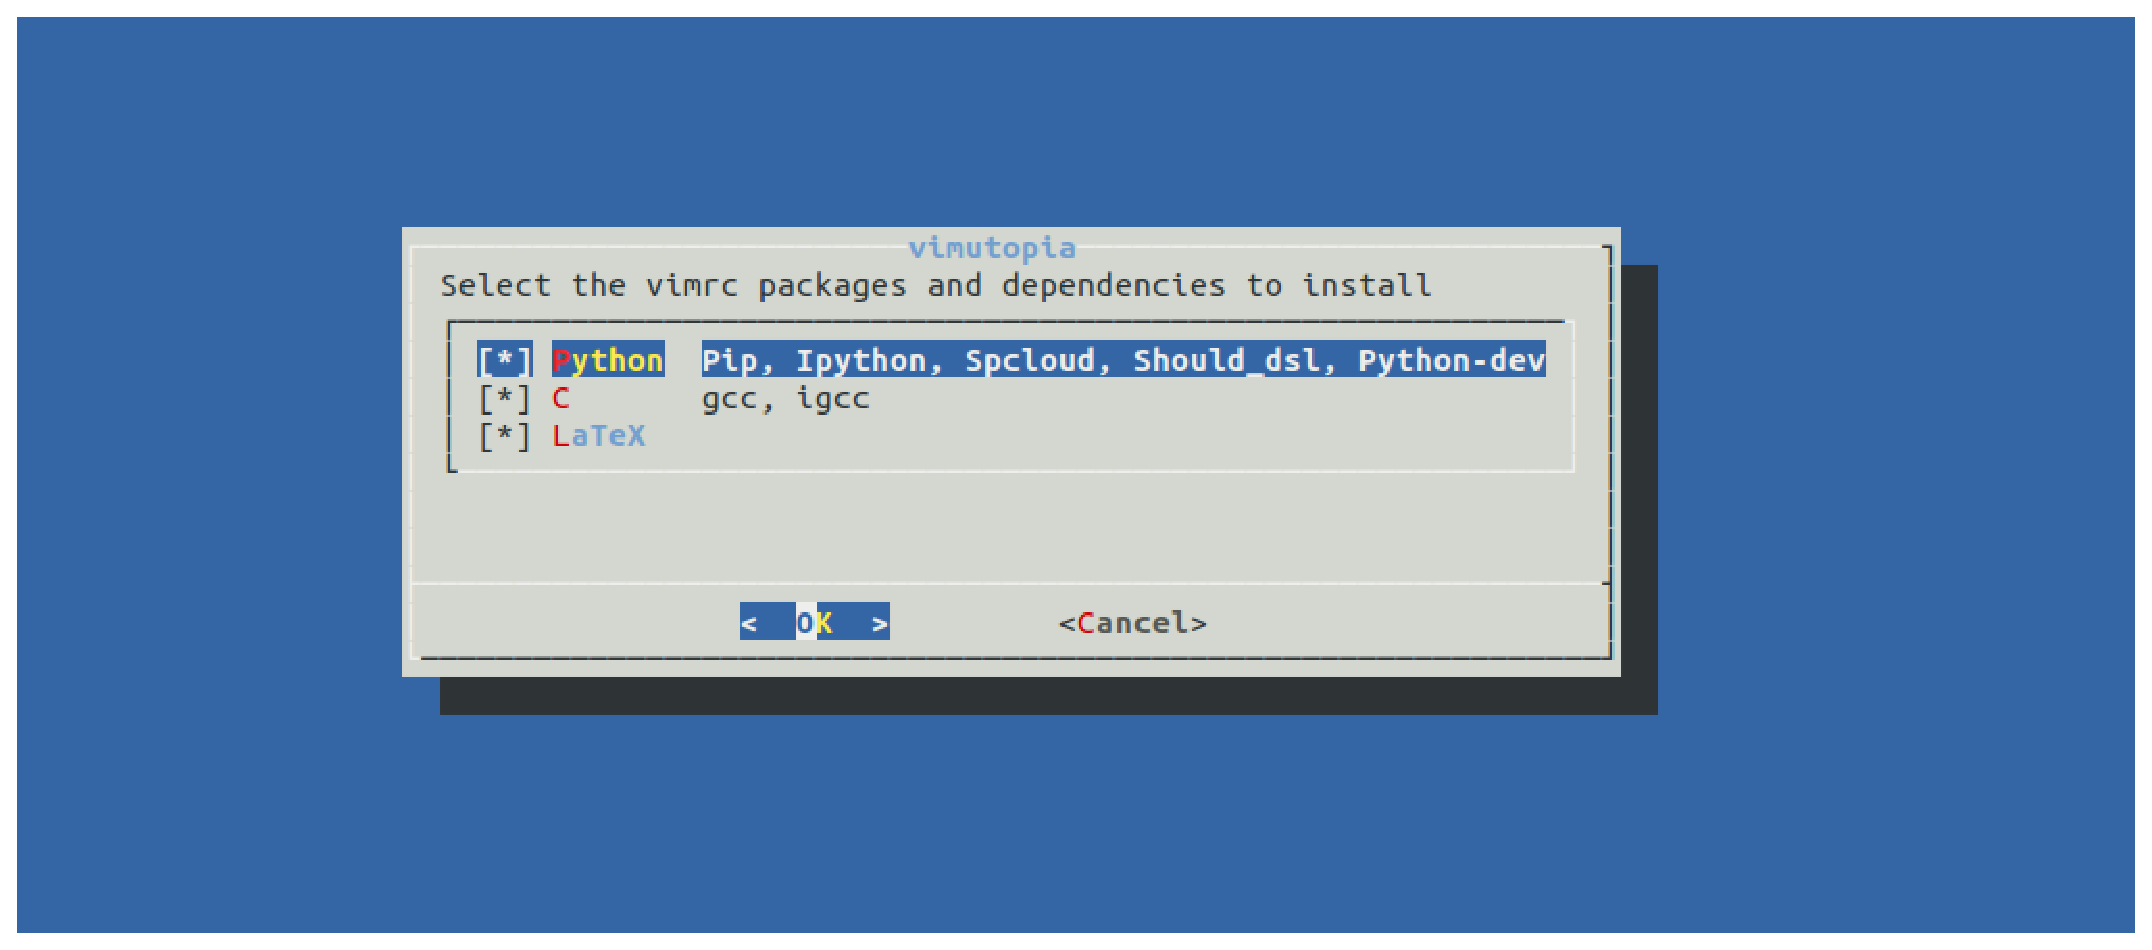
\includegraphics[width=4.5in]{img/install.eps}}
    \end{center}
\end{frame}

\begin{frame}
    \frametitle{Vimutopia}
    \begin{center}
       \framebox{
\includegraphics[width=2in]{img/rocks.eps}}
    \end{center}
\end{frame}
\subsection{Python}

\begin{frame}
    \frametitle{Python}
    \begin{itemize}
        \item<1-> PIP
        \item<2-> Should-dsl
        \item<3-> Specloud
        \item<4-> Ipython
        \item<5-> Atalhos - Specloud, Ipython
    \end{itemize}
\end{frame}

\subsection{C}

\begin{frame}
    \frametitle{C}
    \begin{itemize}
        \item<1-> IGCC
        \item<2-> Atalhos - Roda, Compila
    \end{itemize}
\end{frame}

\subsection{LateX}

\begin{frame}
    \frametitle{LateX}
        Atalhos -  Gera .dvi e .pdf
\end{frame}


\section[Sunshine]{}
\begin{frame}
    \frametitle{Sunshine}
        Não está funfando, mas 'já tem'.
\end{frame}

\subsection{No futuro}

\begin{frame}
    \frametitle{Fuck-yeah}
    \begin{center}
       \framebox{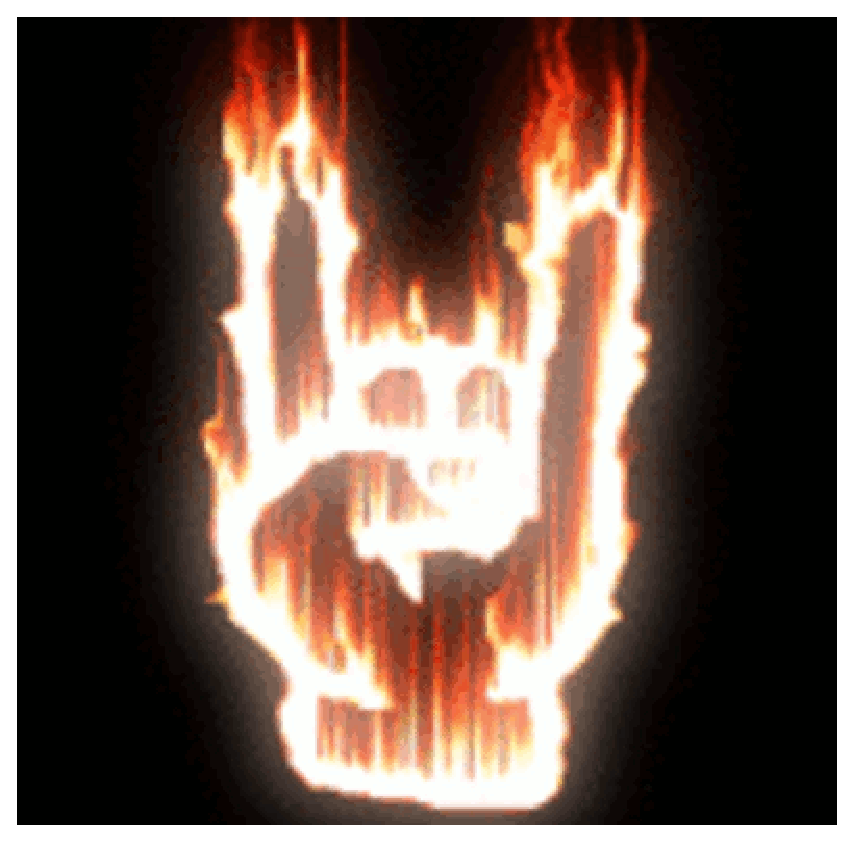
\includegraphics[width=2in]{img/yeah.eps}}
    \end{center}
\end{frame}

\begin{frame}
    \frametitle{No futuro}
    \begin{itemize}
        \item<1-> Pep8 - Adequar código python em tempo real.
        \item<2-> Autocomplete - De acordo com o namespace.
        \item<3-> Documentação - Criar help do uso do Vimutopia.
    \end{itemize}
\end{frame}

\section[Vimutopia]{}

\begin{frame}
    \frametitle{Vimutopia}
             github.com/angelonuffer/Vimutopia
    \begin{center}
       \framebox{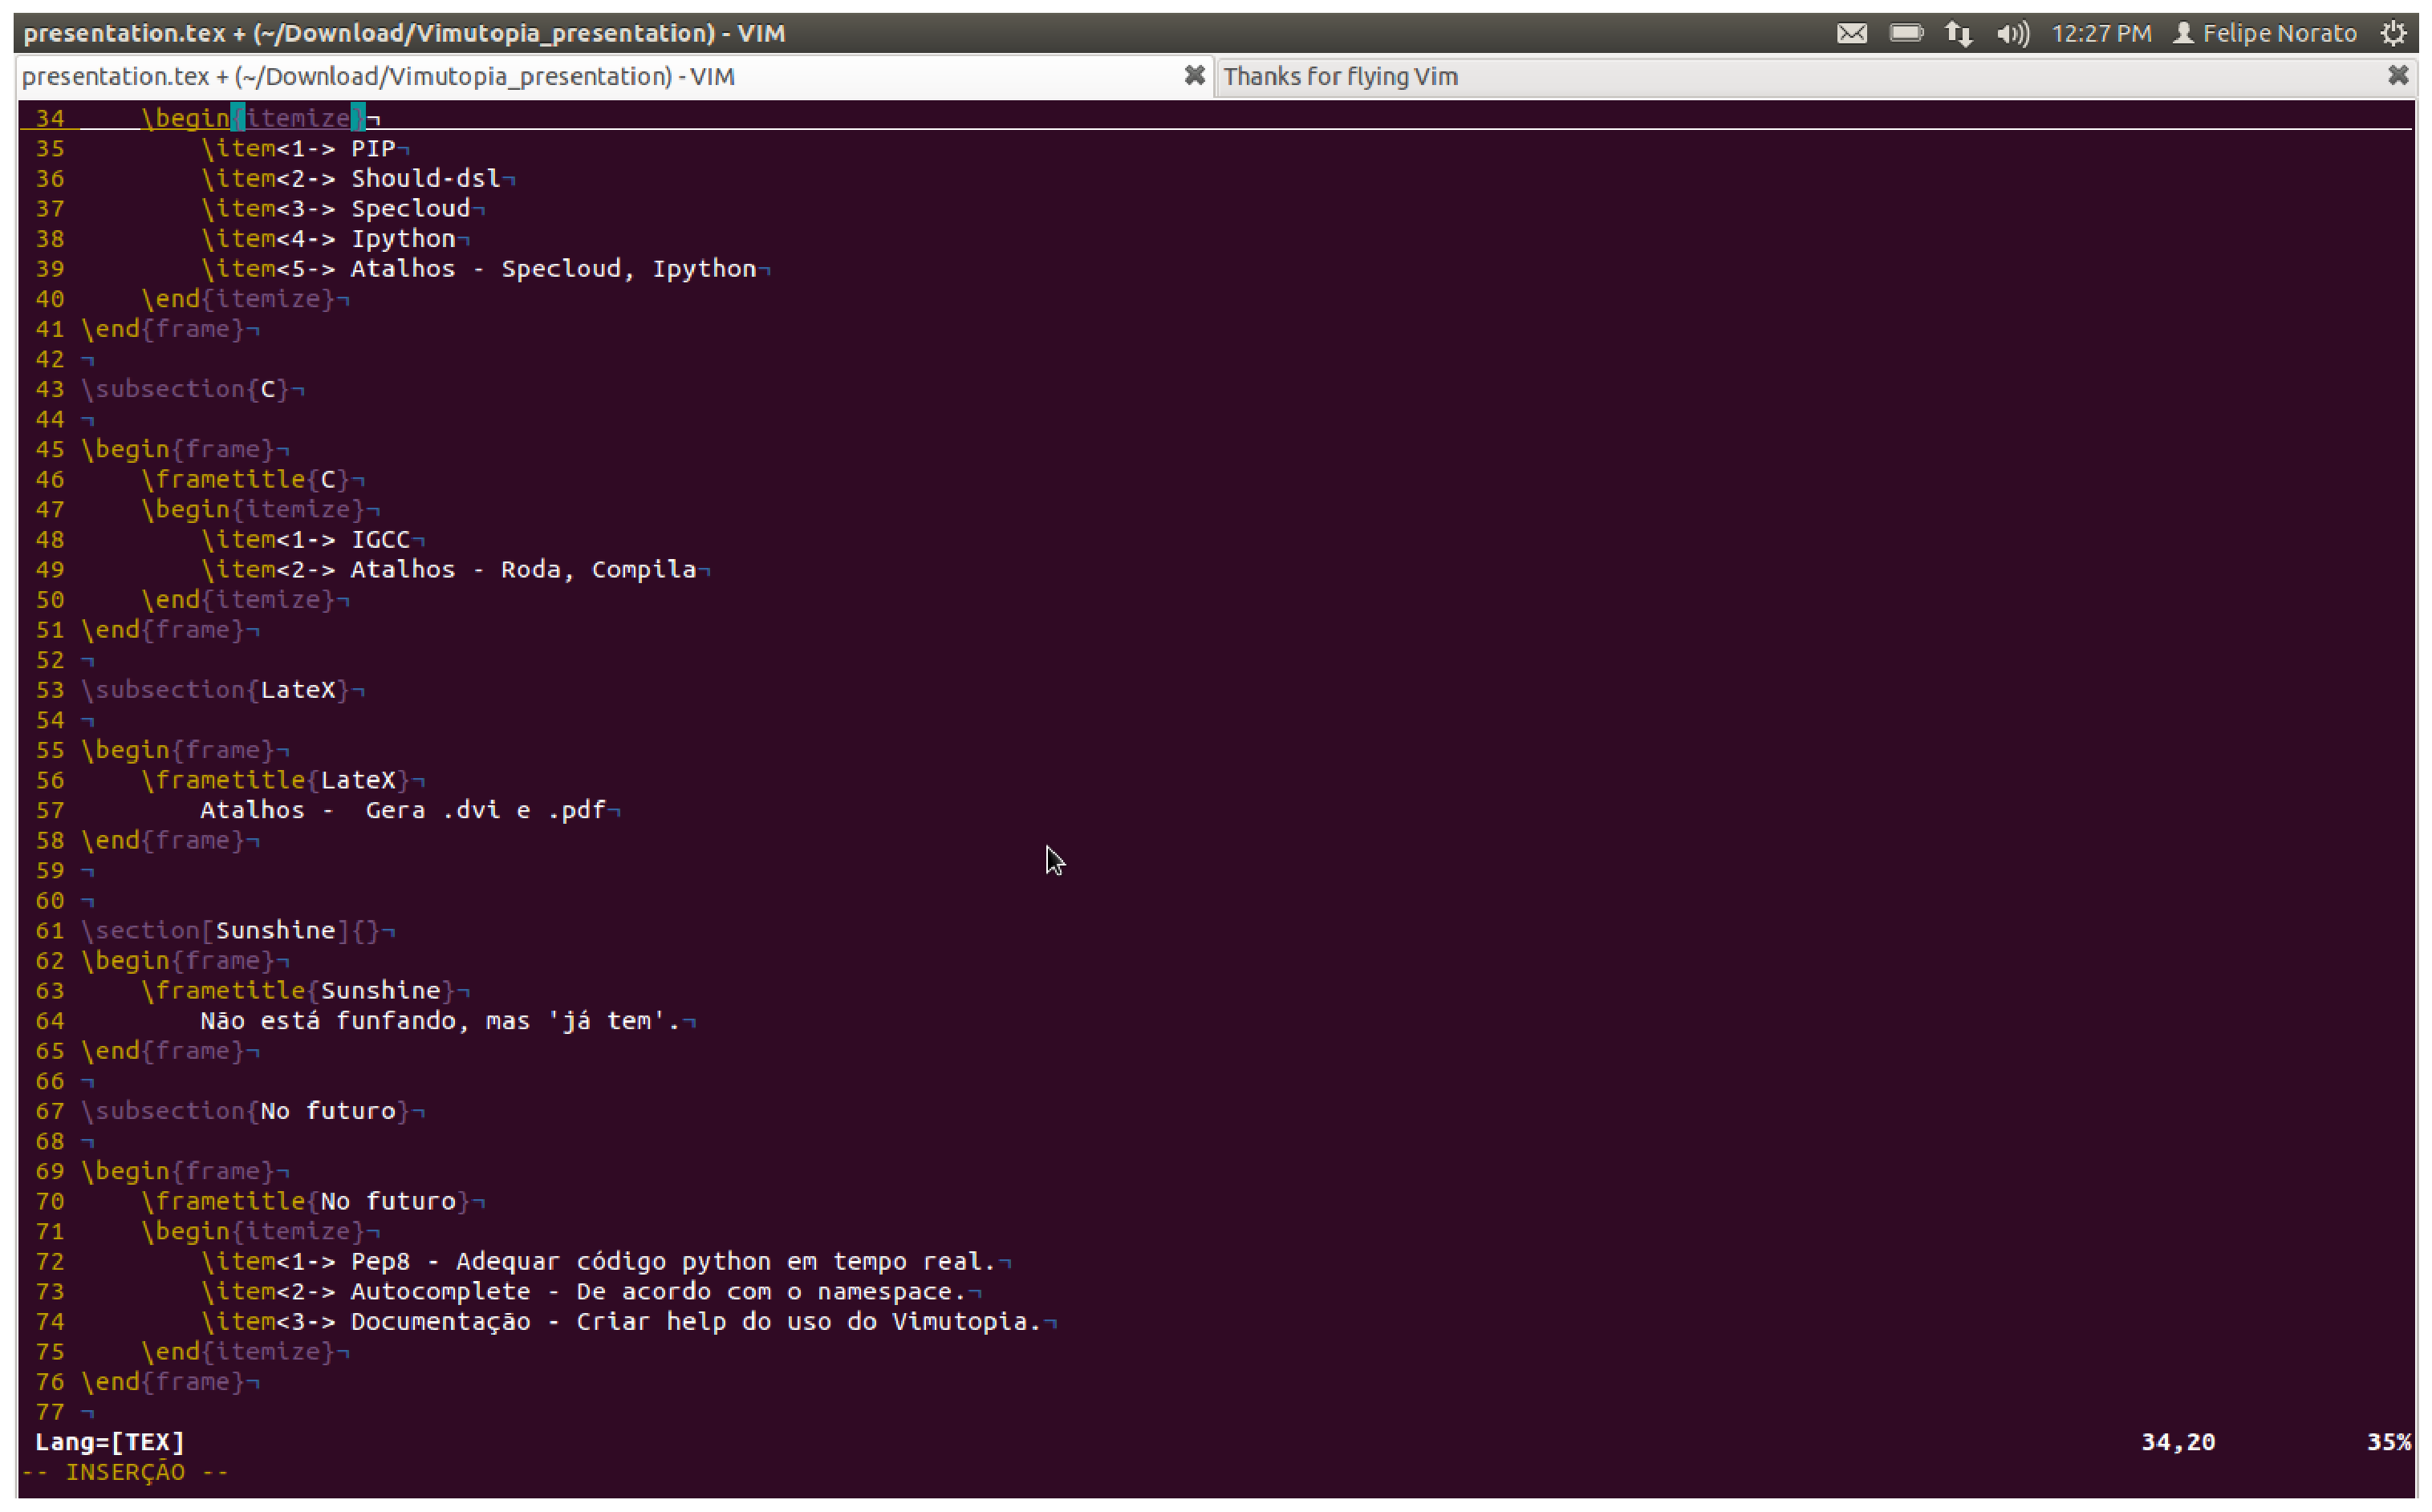
\includegraphics[width=3in]{img/code.eps}}
    \end{center}
\end{frame} 

\section[Perguntas?]{}

\begin{frame}
    \frametitle{Perguntas?}
    \begin{center}
      \framebox{
\includegraphics[width=3in]{img/perguntas.eps}}
    \end{center}
\end{frame}

\begin{frame}
    \frametitle{Obrigado!}
    \begin{itemize}
      \item Angelo Nuffer - github.com/angelonuffer
      \item Felipe Norato - github.com/norato
    \end{itemize}
\end{frame}

\end{document}
